% =============================================================================
%  ASIC Implementation of a Systolic Array Based DNN Accelerator
%  Project I (BECE497J) - Review presentation
%
%  Build:   pdflatex main.tex   (run twice)        images live in ./img/
%  Places to edit are marked with  %%% EDIT %%%
% =============================================================================
\documentclass[aspectratio=169,10pt,t]{beamer}

\usepackage{graphicx}
\usepackage{booktabs}
\usepackage{array}
\usepackage{tabularx}
\usepackage{amsmath,amssymb}
\usepackage{pifont}
\usepackage{tikz}
\usetikzlibrary{arrows.meta,positioning,calc,fit,shapes.geometric,backgrounds}

% ---------- colours ----------
\definecolor{navy}{HTML}{12355B}
\definecolor{teal}{HTML}{1B8A7A}
\definecolor{orange}{HTML}{D9701A}
\definecolor{soft}{HTML}{EEF2F7}
\definecolor{softteal}{HTML}{DFF3EF}
\definecolor{softorange}{HTML}{FCEBDD}
\definecolor{softgrey}{HTML}{F4F4F4}
\definecolor{midgrey}{HTML}{8A8F98}
\definecolor{good}{HTML}{2E8B57}

\setbeamercolor{structure}{fg=navy}
\setbeamercolor{frametitle}{fg=white,bg=navy}
\setbeamercolor{block title}{fg=white,bg=navy}
\setbeamercolor{block body}{fg=black,bg=soft}
\setbeamercolor{itemize item}{fg=teal}
\setbeamercolor{itemize subitem}{fg=teal}
\setbeamerfont{block title}{size=\small,series=\bfseries}
\setbeamerfont{itemize/enumerate body}{size=\small}
\setbeamerfont{itemize/enumerate subbody}{size=\footnotesize}
\setbeamertemplate{navigation symbols}{}
\setbeamertemplate{itemize item}{\small\raisebox{0.1ex}{\textbullet}}
\setbeamersize{text margin left=0.7cm,text margin right=0.7cm}

\setbeamertemplate{frametitle}{%
  \nointerlineskip
  \begin{tikzpicture}[remember picture,overlay]
    \fill[navy] (current page.north west) rectangle ([yshift=-1.05cm]current page.north east);
    \fill[teal] ([yshift=-1.05cm]current page.north west) rectangle ([yshift=-1.12cm]current page.north east);
    \node[anchor=west,text=white,font=\Large\bfseries] at ([xshift=0.7cm,yshift=-0.52cm]current page.north west) {\insertframetitle};
  \end{tikzpicture}\vspace{0.95cm}}

\setbeamertemplate{footline}{%
  \leavevmode\hbox{%
    \begin{beamercolorbox}[wd=.8\paperwidth,ht=2.4ex,dp=1ex,left,leftskip=0.7cm]{footline}
      \tiny\color{midgrey}ASIC Implementation of a Systolic Array Based DNN Accelerator \;|\; Project I (BECE497J)
    \end{beamercolorbox}%
    \begin{beamercolorbox}[wd=.2\paperwidth,ht=2.4ex,dp=1ex,right,rightskip=0.7cm]{footline}
      \tiny\color{midgrey}\insertframenumber\,/\,\inserttotalframenumber
    \end{beamercolorbox}}\vskip0pt}

% ---------- helpers ----------
\newcommand{\py}[1]{\texttt{\detokenize{#1}}}
\newcommand{\ok}{\textcolor{good}{\ding{51}}}
\newcommand{\todo}{\textcolor{orange}{\ding{109}}}
\newcommand{\pend}{\textcolor{midgrey}{\ding{109}}}

% Placeholder for a screenshot the student still has to take.
% usage: \shotbox{height}{caption text}{file name to insert later}
\newcommand{\shotbox}[3]{%
  \begin{tikzpicture}
    \node[draw=orange,dashed,very thick,fill=softorange,minimum width=\linewidth-2pt,minimum height=#1,
          align=center,text width=\linewidth-1cm,font=\footnotesize] {\textbf{INSERT SCREENSHOT HERE}\\[2pt] #2\\[2pt]
          \scriptsize\color{midgrey}(replace this box with \texttt{\textbackslash includegraphics\{img/\detokenize{#3}\}})};
  \end{tikzpicture}}

% Real screenshot with a thin frame.
\graphicspath{{img/}{./}{../img/}}
\newcommand{\shot}[2]{\IfFileExists{img/#2}{\fbox{\includegraphics[width=#1]{img/#2}}}{\IfFileExists{#2}{\fbox{\includegraphics[width=#1]{#2}}}{\fbox{\parbox[c][3cm][c]{#1}{\centering\textcolor{orange}{\textbf{Image not found:}}\\\texttt{\detokenize{#2}}}}}}}

\tikzset{
  blk/.style={draw=navy,fill=soft,rounded corners=2pt,thick,align=center,font=\scriptsize,inner sep=3pt},
  hw/.style={draw=teal,fill=softteal,rounded corners=2pt,thick,align=center,font=\scriptsize,inner sep=3pt},
  sw/.style={draw=orange,fill=softorange,rounded corners=2pt,thick,align=center,font=\scriptsize,inner sep=3pt},
  sim/.style={draw=midgrey,dashed,fill=softgrey,rounded corners=2pt,thick,align=center,font=\scriptsize,inner sep=3pt},
  arr/.style={-{Stealth[length=2.2mm]},thick,navy},
  ctl/.style={-{Stealth[length=2mm]},thick,dashed,orange},
  lab/.style={font=\tiny,midgrey,align=center},
}

\title{ASIC Implementation of a\\Systolic Array Based DNN Accelerator}
\subtitle{Project I (BECE497J) \,--\, Review Presentation}
%%% EDIT %%% put your names and register numbers here
\newcommand{\students}{Vaibhav [Reg.\ No.] \quad [Team member 2] \quad [Team member 3]}
\author{\students}
\institute{Guide: Dr.\ Ravi S\\Vellore Institute of Technology}
\date{October 2026}

\begin{document}

% =============================================================================
\begin{frame}[plain]
  \begin{tikzpicture}[remember picture,overlay]
    \fill[navy] (current page.south west) rectangle (current page.north east);
    \fill[teal] ([yshift=3.1cm]current page.south west) rectangle ([yshift=3.18cm]current page.south east);
    \node[text=white,align=center,font=\bfseries\huge] at ([yshift=-3.2cm]current page.north) {ASIC Implementation of a\\[2pt]Systolic Array Based DNN Accelerator};
    \node[text=white!85!navy,font=\large] at ([yshift=-5.35cm]current page.north) {Project I (BECE497J) \,--\, Review Presentation};
    \node[text=white,align=center,font=\normalsize] at ([yshift=1.7cm]current page.south) {\students\\[3pt]
      Guide: Dr.\ Ravi S \quad|\quad Vellore Institute of Technology \quad|\quad October 2026};
  \end{tikzpicture}
\end{frame}

% =============================================================================
\begin{frame}{Contents}
  \begin{columns}[T]
    \begin{column}{0.48\textwidth}
      \begin{enumerate}\setlength{\itemsep}{3pt}
        \item The project in simple words
        \item Research domain \& problem
        \item Literature survey \& research gap
        \item Objectives \& novelty
        \item System overview (sensor $\to$ host $\to$ chip)
        \item The neural network used
        \item Software / Python flow
      \end{enumerate}
    \end{column}
    \begin{column}{0.48\textwidth}
      \begin{enumerate}\setcounter{enumi}{7}\setlength{\itemsep}{3pt}
        \item Hardware architecture \& data movement
        \item Methodology \& analytical model
        \item Implementation status \& tools
        \item Results: simulation, synthesis, LEC
        \item Tabulation, SDG alignment
        \item Timeline for remaining work
        \item Conclusion \& references
      \end{enumerate}
    \end{column}
  \end{columns}
\end{frame}

% =============================================================================
\begin{frame}{The project in simple words}
  \begin{columns}[T]
    \begin{column}{0.56\textwidth}
      \begin{block}{What problem?}
        \small Recognising something in a picture (here, a handwritten digit) needs millions of
        multiply--add operations. A normal processor does them slowly and uses a lot of energy.
      \end{block}
      \begin{block}{What is our idea?}
        \small Build a \textbf{small dedicated chip} whose only job is these multiply--adds:
        a $4\times4$ grid of 16 tiny calculators working in a rhythm (a \emph{systolic array}).
      \end{block}
      \begin{block}{What have we built so far?}
        \small The complete chip design in Verilog (15 files), the Python tools that train and
        shrink the neural network, a testbench that proves the chip gives the right answers,
        and the synthesis + equivalence-check results.
      \end{block}
    \end{column}
    \begin{column}{0.42\textwidth}
      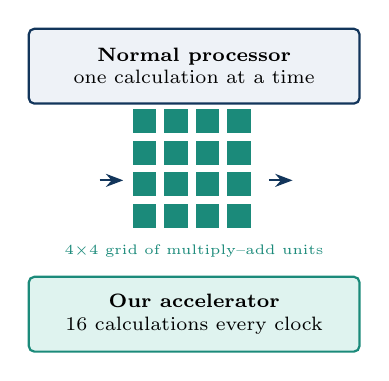
\begin{tikzpicture}[x=1cm,y=1cm]
        \node[blk,minimum width=4.2cm,minimum height=0.95cm] (a) at (0,2.9) {\textbf{Normal processor}\\one calculation at a time};
        \foreach \i in {0,1,2,3}{\foreach \j in {0,1,2,3}{
          \fill[teal] (-0.78+0.4*\i,0.85+0.4*\j) rectangle ++(0.3,0.3);}}
        \draw[arr] (-1.2,1.45) -- ++(0.3,0); \draw[arr] (0.95,1.45) -- ++(0.3,0);
        \node[lab] at (0,0.55) {\textcolor{teal}{4$\times$4 grid of multiply--add units}};
        \node[hw,minimum width=4.2cm,minimum height=0.95cm] (b) at (0,-0.25) {\textbf{Our accelerator}\\16 calculations every clock};
      \end{tikzpicture}
      \vspace{2pt}

      \footnotesize\textbf{In one line:} \emph{we trained a digit-recognising network in Python and designed an ASIC that can run it.}
    \end{column}
  \end{columns}
\end{frame}

% =============================================================================
\begin{frame}{Research domain \& problem focus}
  \begin{columns}[T]
    \begin{column}{0.5\textwidth}
      \begin{block}{Research domain}
        \small VLSI design --- \textbf{hardware accelerators for deep neural network (DNN) inference} at the edge.
      \end{block}
      \begin{block}{Problem}
        \small
        \begin{itemize}\setlength{\itemsep}{1pt}
          \item DNN layers are dominated by \textbf{matrix multiplication} (multiply--accumulate).
          \item On a general CPU these run serially, and fetching data costs more energy than the arithmetic itself.
          \item Edge devices (sensors, wearables) need fast, low-power, \emph{fixed-function} inference.
        \end{itemize}
      \end{block}
    \end{column}
    \begin{column}{0.48\textwidth}
      \begin{block}{Problem focus of this work}
        \small Design, verify and implement (RTL $\to$ GDSII) a \textbf{compact, programmable INT8 systolic-array
        accelerator} that runs a trained network layer by layer, using on-chip data reuse to cut memory traffic,
        and prove it is \textbf{bit-exact} against a Python reference.
      \end{block}
      \begin{block}{Why INT8?}
        \small 8-bit integer multipliers are much smaller and cheaper than 32-bit floating point, and for our network
        cost \textbf{no accuracy} (96.94\% in float, INT8 Python and on the RTL).
      \end{block}
    \end{column}
  \end{columns}
\end{frame}

% =============================================================================
% =============================================================================
%  LITERATURE REVIEW SLIDE (v2): uses only packages already in the preamble.
% =============================================================================
\begin{frame}{Literature review \& research gap identification}
  \scriptsize
  \renewcommand{\arraystretch}{1.35}
  \begin{tabularx}{\textwidth}{@{}p{2.45cm}p{3.35cm}p{2.75cm}>{\raggedright\arraybackslash}X@{}}
    \toprule
    \textcolor{navy}{\textbf{Architecture}} & \textcolor{navy}{\textbf{Dataflow \& precision}} &
    \textcolor{navy}{\textbf{Memory reuse}} & \textcolor{navy}{\textbf{Key limitation in edge AI}}\\
    \midrule
    Google TPU v1\newline(ISCA 2017) & Weight-stationary 256$\times$256,\newline INT8 / 32-bit acc & Unified Buffer (SRAM) &
      Host CISC overhead; low utilisation at small batches ($M{=}1..8$)\\
    Eyeriss\newline(ISSCC 2016) & Row-stationary 14$\times$12,\newline 16-bit fixed point & Global buffer + register files &
      Complex control; large area for local register files\\
    DianNao\newline(ASPLOS 2014) & Central NFU engine,\newline 16-bit fixed point & Multi-banked NBin / SB &
      Routing capacitance; memory-bus contention at scale\\
    Generic edge systolic & Output-stationary,\newline INT8 / FP16 & Streamed from SRAM &
      Re-reads activations; no integrated requantization\\
    \midrule
    \textcolor{teal}{\textbf{Proposed (this work)}} & \textcolor{teal}{\textbf{Weight-stationary 4$\times$4,\newline signed INT8 / 32-bit acc}} &
      \textcolor{teal}{\textbf{LRB + ping-pong SRAM}} &
      \textcolor{teal}{\textbf{Fused PPU; $\approx$74\% fewer activation SRAM reads}}\\
    \bottomrule
  \end{tabularx}

  \vspace{4pt}
  \begin{block}{Research gaps addressed by this project}
    \scriptsize
    \renewcommand{\arraystretch}{1.25}
    \begin{tabularx}{\textwidth}{@{}p{3.9cm}>{\raggedright\arraybackslash}X@{}}
      \textbf{1. Redundant activation re-reads} & tiled arrays re-fetch the same activations for every column tile $\Rightarrow$ \textbf{Local Reuse Buffer}\\
      \textbf{2. Per-layer host scheduling} & CPU reprograms pointers layer by layer $\Rightarrow$ \textbf{autonomous descriptor FSM}\\
      \textbf{3. Post-processing round-trips} & bias, scaling, ReLU go back to main memory $\Rightarrow$ \textbf{fused 3-stage PPU}\\
      \textbf{4. Sign and overflow pitfalls} & unsigned PEs break signed weights; short accumulators overflow $\Rightarrow$ \textbf{signed INT8, 32-bit accumulation}\\
    \end{tabularx}
  \end{block}
\end{frame}


% =============================================================================
\begin{frame}{Objectives \& novelty of the work}
  \begin{columns}[T]
    \begin{column}{0.4\textwidth}
      \begin{block}{Objectives}
        \footnotesize
        \begin{enumerate}\setlength{\itemsep}{2pt}
          \item Design a weight-stationary INT8 systolic array accelerator in synthesizable Verilog.
          \item Make it \emph{programmable}: network = data loaded at run time.
          \item Reduce SRAM traffic with a local reuse buffer.
          \item Prove correctness against a bit-exact Python model.
          \item Synthesize and formally check the netlist; take the design towards GDSII.
        \end{enumerate}
      \end{block}
      \scriptsize\emph{Novelty lies in the integration, the reuse buffer and the verified open flow --- not in a new algorithm.}
    \end{column}
    \begin{column}{0.58\textwidth}
      \begin{block}{What is novel / different}
        \footnotesize
        \begin{itemize}\setlength{\itemsep}{2pt}
          \item \textbf{Network is data, not hardware}: layer descriptors + weights are loaded into SRAM; same chip runs other dense networks.
          \item \textbf{Local Reuse Buffer (LRB)}: activation SRAM reads per batch fall from \textbf{608 to 160} (3.8$\times$); 74\% of activation fetches served on-chip.
          \item \textbf{INT8 end to end on chip}: accumulation, bias, rescale and ReLU are done in hardware; the host does no maths between layers.
          \item \textbf{Complete open flow} from PyTorch to register program, verified bit-exact.
          \item \textbf{Host-ready}: register bus + AXI4-Lite bridge, C driver, hardware performance counters.
        \end{itemize}
      \end{block}
    \end{column}
  \end{columns}
\end{frame}

% =============================================================================
\begin{frame}{System overview: how it works in the real world}
  \centering
  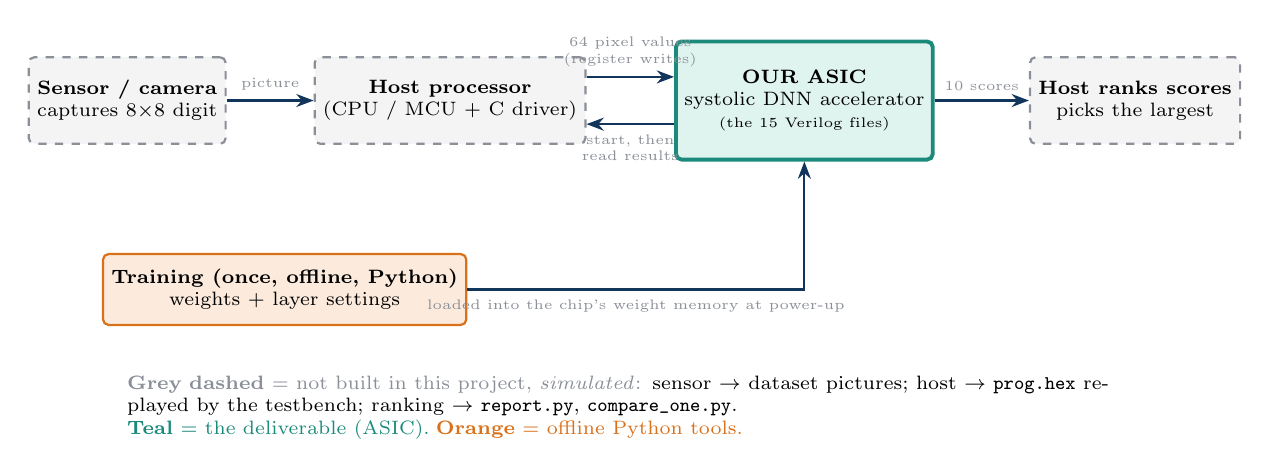
\begin{tikzpicture}[x=1cm,y=1cm]
    \node[sim,minimum width=2.5cm,minimum height=1.1cm] (sen) at (0,0) {\textbf{Sensor / camera}\\captures 8$\times$8 digit};
    \node[sim,minimum width=2.7cm,minimum height=1.1cm] (host) at (4.1,0) {\textbf{Host processor}\\(CPU / MCU + C driver)};
    \node[hw,minimum width=3.0cm,minimum height=1.5cm,line width=1.4pt] (chip) at (8.6,0) {\textbf{OUR ASIC}\\systolic DNN accelerator\\{\tiny (the 15 Verilog files)}};
    \node[sim,minimum width=2.2cm,minimum height=1.1cm] (res) at (12.8,0) {\textbf{Host ranks scores}\\picks the largest};
    \draw[arr] (sen) -- node[above,lab]{picture} (host);
    \draw[arr] ([yshift=0.3cm]host.east) -- node[above,lab]{64 pixel values\\(register writes)} ([yshift=0.3cm]chip.west);
    \draw[arr] ([yshift=-0.3cm]chip.west) -- node[below,lab]{start, then\\read results} ([yshift=-0.3cm]host.east);
    \draw[arr] (chip.east) -- node[above,lab]{10 scores} (res.west);
    % one time loading
    \node[sw,minimum width=4.6cm,minimum height=0.9cm] (train) at (2.0,-2.4) {\textbf{Training (once, offline, Python)}\\weights + layer settings};
    \draw[arr] (train.east) -| node[pos=0.25,below,lab]{loaded into the chip's weight memory at power-up} (chip.south);
    \node[lab,align=center] at (6.7,-2.95) {};
    % what is simulated
    \node[font=\scriptsize,align=left,text width=12.8cm] at (6.4,-3.9)
      {\textcolor{midgrey}{\textbf{Grey dashed} = not built in this project, \emph{simulated}:} sensor $\to$ dataset pictures;
       host $\to$ \py{prog.hex} replayed by the testbench; ranking $\to$ \py{report.py}, \py{compare_one.py}.\\
       \textcolor{teal}{\textbf{Teal} = the deliverable (ASIC).}\;\textcolor{orange}{\textbf{Orange} = offline Python tools.}};
  \end{tikzpicture}
  \vspace{-4pt}
\end{frame}

% =============================================================================
\begin{frame}{The neural network used: digit recognition}
  \begin{columns}[T]
    \begin{column}{0.58\textwidth}
      \centering
      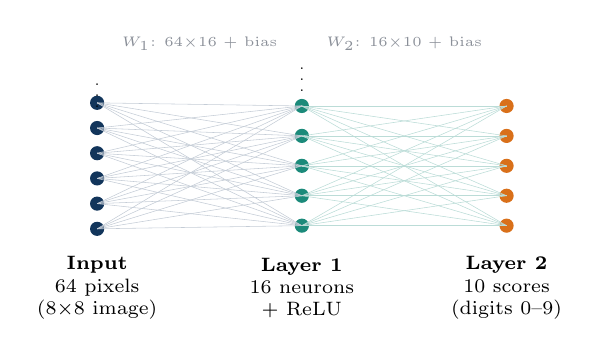
\begin{tikzpicture}[x=1cm,y=1cm]
        % layers
        \foreach \i in {0,...,5}{\fill[navy] (0,\i*0.32-0.8) circle (0.09);}
        \node[font=\tiny] at (0,1.0) {\vdots};
        \foreach \i in {0,...,4}{\fill[teal] (2.6,\i*0.38-0.76) circle (0.09);}
        \node[font=\tiny] at (2.6,1.2) {\vdots};
        \foreach \i in {0,...,4}{\fill[orange] (5.2,\i*0.38-0.76) circle (0.09);}
        \foreach \i in {0,...,5}{\foreach \j in {0,...,4}{\draw[navy!25,very thin] (0,\i*0.32-0.8)--(2.6,\j*0.38-0.76);}}
        \foreach \i in {0,...,4}{\foreach \j in {0,...,4}{\draw[teal!30,very thin] (2.6,\i*0.38-0.76)--(5.2,\j*0.38-0.76);}}
        \node[font=\scriptsize,align=center] at (0,-1.55) {\textbf{Input}\\64 pixels\\(8$\times$8 image)};
        \node[font=\scriptsize,align=center] at (2.6,-1.55) {\textbf{Layer 1}\\16 neurons\\+ ReLU};
        \node[font=\scriptsize,align=center] at (5.2,-1.55) {\textbf{Layer 2}\\10 scores\\(digits 0--9)};
        \node[lab] at (1.3,1.55) {$W_1$: 64$\times$16 + bias};
        \node[lab] at (3.9,1.55) {$W_2$: 16$\times$10 + bias};
      \end{tikzpicture}

      \vspace{4pt}
      \footnotesize Shapes for a batch of 8 pictures: $8{\times}64 \to 8{\times}16 \to 8{\times}10$.\\
      1,184 weights + 26 biases in total.
    \end{column}
    \begin{column}{0.4\textwidth}
      \small
      \begin{block}{Dataset}
        \footnotesize UCI \emph{Optical Recognition of Handwritten Digits} (Alpaydin \& Kaynak, 1998), loaded through scikit-learn.
        1,797 images of 8$\times$8 pixels.\\[2pt]
        \textbf{1,437} for training, \textbf{360} held back for testing (fixed split, stratified).
      \end{block}
      \begin{block}{How a digit is decided}
        \footnotesize The chip outputs 10 scores; the \textbf{largest score is the predicted digit}.
        Example: $[-12,4,-7,\mathbf{91},-30,\dots]\Rightarrow 3$.
      \end{block}
    \end{column}
  \end{columns}
\end{frame}

% =============================================================================
\begin{frame}{Software flow: the Python scripts and what they do}
  \centering
  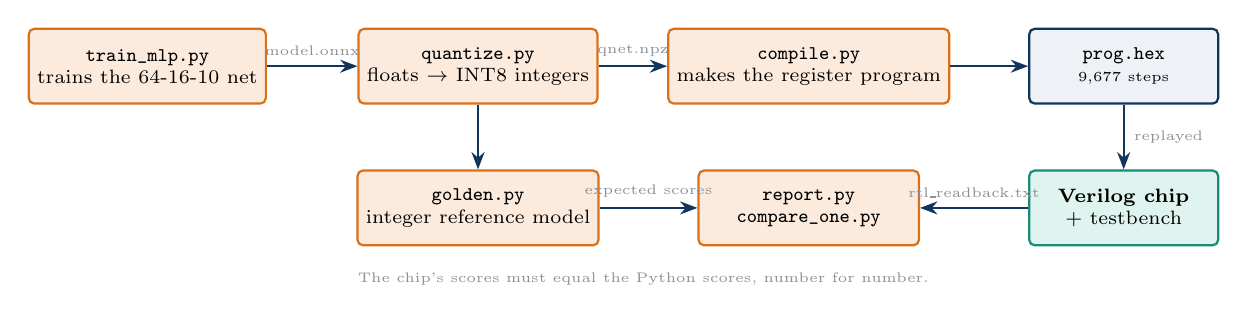
\begin{tikzpicture}[x=1cm,y=1cm]
    \node[sw,minimum width=2.8cm,minimum height=0.95cm] (t) at (0,0) {\py{train_mlp.py}\\trains the 64-16-10 net};
    \node[sw,minimum width=2.8cm,minimum height=0.95cm] (q) at (4.2,0) {\py{quantize.py}\\floats $\to$ INT8 integers};
    \node[sw,minimum width=2.8cm,minimum height=0.95cm] (c) at (8.4,0) {\py{compile.py}\\makes the register program};
    \node[blk,minimum width=2.4cm,minimum height=0.95cm] (p) at (12.4,0) {\py{prog.hex}\\{\tiny 9,677 steps}};
    \draw[arr] (t) -- node[above,lab]{model.onnx} (q);
    \draw[arr] (q) -- node[above,lab]{qnet.npz} (c);
    \draw[arr] (c) -- (p);
    \node[sw,minimum width=2.8cm,minimum height=0.95cm] (g) at (4.2,-1.8) {\py{golden.py}\\integer reference model};
    \node[sw,minimum width=2.8cm,minimum height=0.95cm] (r) at (8.4,-1.8) {\py{report.py}\\\py{compare_one.py}};
    \node[hw,minimum width=2.4cm,minimum height=0.95cm] (chip) at (12.4,-1.8) {\textbf{Verilog chip}\\+ testbench};
    \draw[arr] (p) -- node[right,lab]{replayed} (chip);
    \draw[arr] (chip) -- node[above,lab]{rtl\_readback.txt} (r);
    \draw[arr] (q) -- (g);
    \draw[arr] (g) -- node[above,lab]{expected scores} (r);
    \node[lab] at (6.3,-2.7) {The chip's scores must equal the Python scores, number for number.};
  \end{tikzpicture}
  \vspace{-2pt}

  \scriptsize
  \renewcommand{\arraystretch}{1.05}
  \begin{tabularx}{\textwidth}{@{}>{\ttfamily}p{3.0cm}X@{}}
    \toprule
    \textbf{Script} & \textbf{Job (in simple words)}\\
    \midrule
    train\_mlp.py & Trains the network on 1,437 pictures (PyTorch); saves the weights (ONNX).\\
    quantize.py & Converts decimal weights into small 8-bit integers + works out the multiply/shift numbers.\\
    compile.py & Acts like the host driver: writes the list of register writes that loads weights, sends pictures, starts the chip, reads scores.\\
    golden.py & Same arithmetic in plain integer Python --- the ``answer key'' the chip must match exactly.\\
    report.py, compare\_one.py & Read the chip's output, pick the biggest score per picture, compute accuracy; show chip vs Python side by side.\\
    show\_digits.py & Displays the actual test pictures in a browser.\\
    \bottomrule
  \end{tabularx}
\end{frame}

% =============================================================================
\begin{frame}{Functional block diagram of the accelerator}
  \centering
  \resizebox{0.98\textwidth}{!}{%
  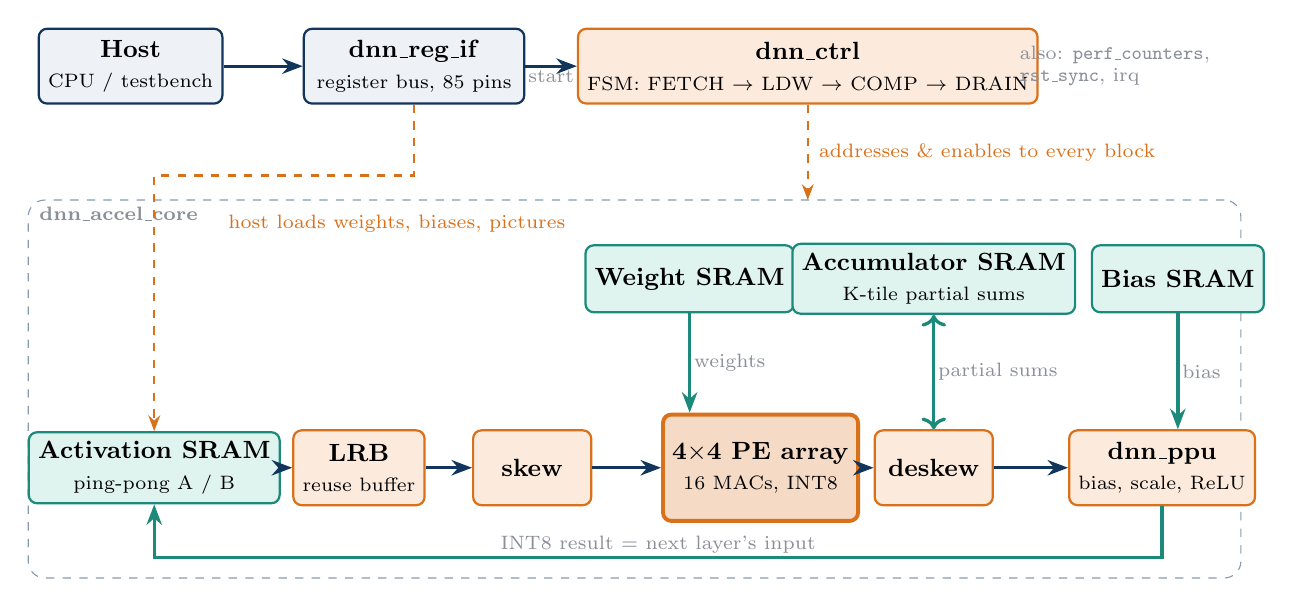
\begin{tikzpicture}[x=1cm,y=1cm,
      bx/.style={draw=navy,rounded corners=3pt,fill=soft,thick,align=center,minimum height=0.95cm,font=\small},
      mem/.style={draw=teal,rounded corners=3pt,fill=softteal,thick,align=center,minimum height=0.85cm,minimum width=2.3cm,font=\small},
      cmp/.style={draw=orange,rounded corners=3pt,fill=softorange,thick,align=center,minimum height=0.95cm,font=\small},
      df/.style={-{Stealth[length=2.6mm]},very thick,navy},
      cl/.style={-{Stealth[length=2mm]},thick,dashed,orange},
      tl/.style={font=\scriptsize,text=midgrey,inner sep=1pt}]
    % ---- host side ----
    \node[bx,minimum width=2.2cm] (host) at (0.4,5.3) {\textbf{Host}\\{\scriptsize CPU / testbench}};
    \node[bx,minimum width=2.8cm] (rif) at (4.0,5.3) {\textbf{dnn\_reg\_if}\\{\scriptsize register bus, 85 pins}};
    \node[bx,minimum width=4.4cm,fill=softorange,draw=orange] (ctrl) at (9.0,5.3) {\textbf{dnn\_ctrl}\\{\scriptsize FSM: FETCH $\to$ LDW $\to$ COMP $\to$ DRAIN}};
    \node[tl,align=left] at (12.9,5.3) {also: \texttt{perf\_counters},\\\texttt{rst\_sync}, irq};
    \draw[df] (host) -- (rif);
    \draw[df] (rif) -- node[below,tl]{start} (ctrl);
    % ---- core frame ----
    \begin{scope}[on background layer]
      \node[draw=navy!50,dashed,rounded corners=6pt,fill=white,fit={(-0.9,-1.2) (14.5,3.6)},inner sep=0pt] (core) {};
    \end{scope}
    \node[tl,anchor=north west] at (-0.8,3.55) {\textbf{dnn\_accel\_core}};
    % ---- memories row ----
    \node[mem,minimum width=2.0cm] (wm) at (7.5,2.6) {\textbf{Weight SRAM}};
    \node[mem,minimum width=2.4cm] (acc) at (10.6,2.6) {\textbf{Accumulator SRAM}\\{\scriptsize K-tile partial sums}};
    \node[mem,minimum width=1.6cm] (bm) at (13.7,2.6) {\textbf{Bias SRAM}};
    % ---- datapath row ----
    \node[mem,minimum width=2.4cm] (am) at (0.7,0.2) {\textbf{Activation SRAM}\\{\scriptsize ping-pong A / B}};
    \node[cmp,minimum width=1.5cm] (lrb) at (3.3,0.2) {\textbf{LRB}\\{\scriptsize reuse buffer}};
    \node[cmp,minimum width=1.5cm] (sk) at (5.5,0.2) {\textbf{skew}};
    \node[cmp,minimum width=2.3cm,minimum height=1.35cm,line width=1.4pt,fill=orange!25] (pe) at (8.4,0.2) {\textbf{4$\times$4 PE array}\\{\scriptsize 16 MACs, INT8}};
    \node[cmp,minimum width=1.5cm] (dsk) at (10.6,0.2) {\textbf{deskew}};
    \node[cmp,minimum width=1.9cm] (ppu) at (13.5,0.2) {\textbf{dnn\_ppu}\\{\scriptsize bias, scale, ReLU}};
    \draw[df] (am) -- (lrb); \draw[df] (lrb) -- (sk); \draw[df] (sk) -- (pe); \draw[df] (pe) -- (dsk); \draw[df] (dsk) -- (ppu);
    \draw[df,teal] (wm.south) -- node[right,tl]{weights} (wm.south |- pe.north);
    \draw[df,teal,<->] (acc.south) -- node[right,tl]{partial sums} (acc.south |- dsk.north);
    \draw[df,teal] (bm.south) -- node[right,tl]{bias} (bm.south |- ppu.north);
    % write-back
    \draw[df,teal] (ppu.south) -- ++(0,-0.65) -| node[pos=0.25,above,tl]{INT8 result = next layer's input} (am.south);
    % control
    \draw[cl] (ctrl.south) -- (9.0,3.6);
    \node[tl,text=orange,anchor=west] at (9.1,4.2) {addresses \& enables to every block};
    \draw[cl] (rif.south) -- ++(0,-0.9) -| (am.north) ;
    \node[tl,text=orange,anchor=west] at (1.6,3.3) {host loads weights, biases, pictures};
  \end{tikzpicture}}
  \vspace{-2pt}

  \footnotesize\textbf{Reading it:} data flows left to right along the bottom row (pictures $\to$ array $\to$ result); weights, partial sums and biases join from the memories above; the controller sequences everything. 15 Verilog files in total.
\end{frame}

% =============================================================================
\begin{frame}{Local Reuse Buffer (LRB): why it exists and how it works}
  \centering
  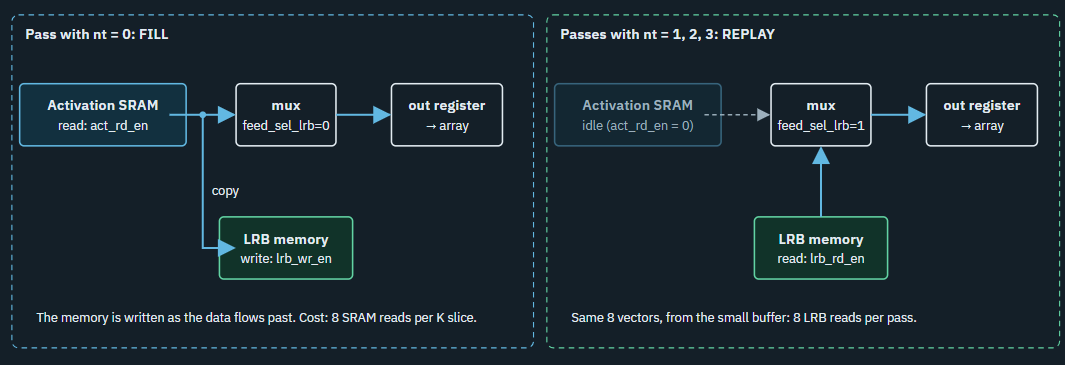
\includegraphics[width=0.97\textwidth]{img/lrb_fill_replay_crop.png}

  \vspace{3pt}
  \begin{columns}[T]
    \begin{column}{0.33\textwidth}
      \small\textbf{Problem.} A layer is cut into tiles; every column tile ($nt$) needs the \emph{same} activations again.
    \end{column}
    \begin{column}{0.33\textwidth}
      \small\textbf{Idea.} First tile: read the SRAM and copy to the LRB. Other tiles: replay from the small LRB; the SRAM stays idle.
    \end{column}
    \begin{column}{0.33\textwidth}
      \small\textbf{Result.} SRAM reads per batch: \textbf{608 $\to$ 160} ($-73.7\%$); measured = analytical $(NT-1)/NT$.
    \end{column}
  \end{columns}
\end{frame}

% =============================================================================
\begin{frame}{The processing element and the systolic array}
  \begin{columns}[T]
    \begin{column}{0.52\textwidth}
      \centering
      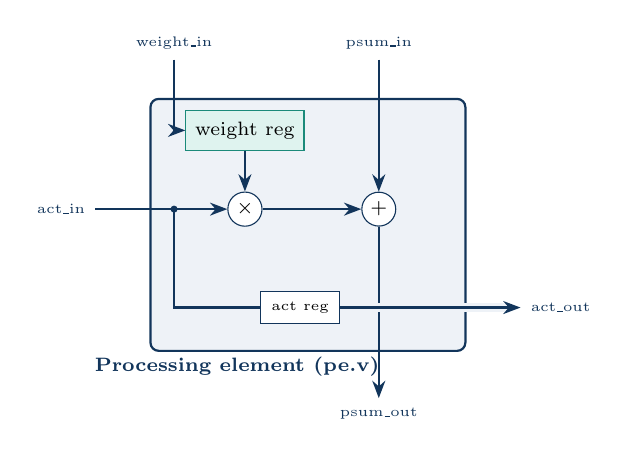
\begin{tikzpicture}[x=1cm,y=1cm]
        \node[draw=navy,thick,fill=soft,minimum width=4.0cm,minimum height=3.2cm,rounded corners=3pt] at (0,-0.4) {};
        \node[font=\scriptsize\bfseries,navy] at (-0.9,-2.2) {Processing element (pe.v)};
        \node[draw=teal,fill=softteal,minimum width=1.5cm,minimum height=0.5cm,font=\scriptsize] (w) at (-0.8,0.8) {weight reg};
        \node[draw=navy,fill=white,circle,font=\scriptsize,inner sep=1.5pt] (mul) at (-0.8,-0.2) {$\times$};
        \node[draw=navy,fill=white,circle,font=\scriptsize,inner sep=1.5pt] (add) at (0.9,-0.2) {$+$};
        \node[draw=navy,fill=white,minimum width=1.0cm,minimum height=0.4cm,font=\tiny] (ar) at (-0.1,-1.45) {act reg};
        \draw[arr] (w) -- (mul);
        \draw[arr] (mul) -- (add);
        % psum vertical
        \draw[arr] (0.9,1.7) node[above,font=\tiny]{psum\_in} -- (add.north);
        \draw[arr] (add.south) -- (0.9,-2.6) node[below,font=\tiny]{psum\_out};
        % act horizontal
        \draw[navy,thick] (-2.7,-0.2) node[left,font=\tiny]{act\_in} -- (-1.7,-0.2) coordinate (br);
        \draw[arr] (br) -- (mul.west);
        \fill[navy] (br) circle (0.045);
        \draw[navy,thick] (br) |- (ar.west);
        \draw[arr,preaction={draw=soft,line width=3.2pt}] (ar.east) -- (2.7,-1.45) node[right,font=\tiny]{act\_out};
        \draw[arr] (-1.7,1.7) node[above,font=\tiny]{weight\_in} -- (-1.7,0.8) -- (w.west);
      \end{tikzpicture}

      \vspace{2pt}
      \scriptsize Signed INT8 $\times$ INT8 $\to$ 16-bit product, summed in a 32-bit accumulator.
    \end{column}
    \begin{column}{0.46\textwidth}
      \centering
      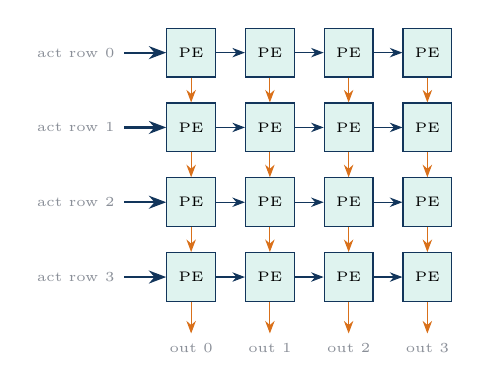
\begin{tikzpicture}[x=1cm,y=1cm]
        \foreach \r in {0,1,2,3}{
          \foreach \c in {0,1,2,3}{
            \node[draw=navy,fill=softteal,minimum size=0.62cm,font=\tiny] (p\r\c) at (\c*1.0,-\r*0.95) {PE};
          }}
        \foreach \r in {0,1,2,3}{
          \draw[arr] (-0.85,-\r*0.95) -- (p\r0.west);
          \foreach \c in {0,1,2}{\pgfmathtruncatemacro{\n}{\c+1}\draw[-{Stealth[length=1.6mm]},navy] (p\r\c.east) -- (p\r\n.west);}
          \node[lab,left] at (-0.85,-\r*0.95) {act row \r};
        }
        \foreach \c in {0,1,2,3}{
          \foreach \r in {0,1,2}{\pgfmathtruncatemacro{\n}{\r+1}\draw[-{Stealth[length=1.6mm]},orange] (p\r\c.south) -- (p\n\c.north);}
          \draw[-{Stealth[length=1.6mm]},orange] (p3\c.south) -- ++(0,-0.4) node[below,lab]{out \c};
        }
      \end{tikzpicture}

      \vspace{2pt}
      \footnotesize
      \begin{align*}
        \texttt{psum\_out} &\leftarrow \texttt{psum\_in} + \texttt{weight}\times\texttt{act\_in}\\
        \texttt{act\_out} &\leftarrow \texttt{act\_in}
      \end{align*}
      \scriptsize
      \textcolor{navy}{$\rightarrow$ activations move right}, \textcolor{orange}{$\downarrow$ partial sums move down}.\\
      Weights stay in place (\textbf{weight-stationary}).\\
      Each column adds 4 products = one dot product.
    \end{column}
  \end{columns}
\end{frame}

% =============================================================================
\begin{frame}{How data moves: one batch through the chip}
  \begin{columns}[T]
    \begin{column}{0.52\textwidth}
      \footnotesize
      \begin{enumerate}\setlength{\itemsep}{1.5pt}
        \item \textbf{Tile:} the $64{\times}16$ weight matrix is cut into $4{\times}4$ tiles (64 for layer 1, 12 for layer 2).
        \item \textbf{Load} one tile's weights down the columns; they stay put.
        \item \textbf{Stream} 8 pictures through; \emph{skew} delays row $r$ by $r$ clocks so each activation meets the right partial sum.
        \item \textbf{Reuse:} the first pass fills the \emph{LRB}; later passes replay from it instead of re-reading SRAM.
        \item \textbf{Accumulate} the partial sums of all tiles in the accumulator SRAM.
        \item \textbf{Post-process (PPU):} bias, scale, round, ReLU, clamp to INT8.
        \item \textbf{Ping-pong:} layer 1's output is written to the other half of the activation memory = layer 2's input.
      \end{enumerate}
    \end{column}
    \begin{column}{0.44\textwidth}
      \centering
      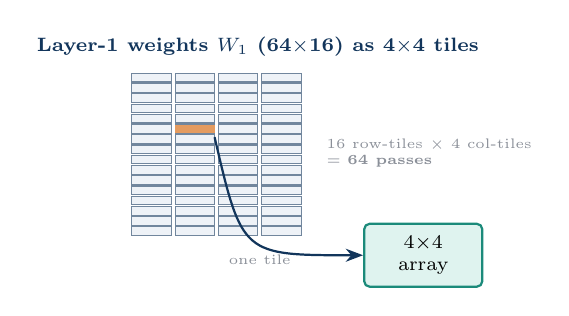
\begin{tikzpicture}[x=1cm,y=1cm]
        \node[font=\scriptsize\bfseries,navy] at (1.6,0.35) {Layer-1 weights $W_1$ (64$\times$16) as 4$\times$4 tiles};
        \foreach \i in {0,...,15}{\foreach \j in {0,...,3}{
          \draw[navy!60,fill=soft] (\j*0.55,-0.1-\i*0.13) rectangle ++(0.5,0.11);}}
        \fill[orange!70] (0.55,-0.1-5*0.13) rectangle ++(0.5,0.11);
        \node[lab,right,align=left] at (2.35,-1.0) {16 row-tiles $\times$ 4 col-tiles\\= \textbf{64 passes}};
        \node[hw,minimum width=1.5cm,minimum height=0.8cm] (arr) at (3.7,-2.3) {4$\times$4\\array};
        \draw[arr] (1.05,-0.1-5*0.13-0.05) .. controls (1.4,-2.3) .. (arr.west) node[pos=0.55,below,lab]{one tile};
      \end{tikzpicture}

      \vspace{2pt}
      \footnotesize
      \begin{tabular}{@{}lr@{}}
        \toprule
        \textbf{Per batch of 8 pictures} & \\
        \midrule
        Layer 1 passes & 64\\
        Layer 2 passes & 12\\
        \textbf{Total passes} & \textbf{76}\\
        Clock cycles (measured) & 1,771\\
        Cycles per picture & 221\\
        \bottomrule
      \end{tabular}
    \end{column}
  \end{columns}
\end{frame}

% =============================================================================
\begin{frame}{Algorithm and analytical model}
  \begin{columns}[T]
    \begin{column}{0.52\textwidth}
      \begin{block}{1. Layer maths (what the array computes)}
        \small $y_n=\displaystyle\sum_{k} x_k\,w_{k,n}+b_n$
      \end{block}
      \begin{block}{2. INT8 model (what the chip implements)}
        \small
        \begin{align*}
          acc_n &= \textstyle\sum_k x^{q}_k\,w^{q}_{k,n} \quad(\text{32-bit})\\
          y^{q}_n &= \operatorname{clamp}\!\Big(\big((acc_n+b^{q}_n)\cdot m + 2^{s-1}\big)\gg s,\ lo,\ 127\Big)
        \end{align*}
        \footnotesize $m$ = multiplier, $s$ = shift, $lo=0$ with ReLU else $-128$. No floating point anywhere, so any mismatch with the RTL is a real bug.
      \end{block}
    \end{column}
    \begin{column}{0.46\textwidth}
      \begin{block}{3. Performance model}
        \small $\text{images/s}=\dfrac{f_{clk}\cdot B}{\text{cycles/batch}}=\dfrac{100\,\text{MHz}\cdot 8}{1771}\approx 4.5\times10^{5}$\\[3pt]
        \footnotesize MACs per picture = $64{\cdot}16+16{\cdot}10 = 1184$; peak = 16 MAC/clock; achieved $\approx$ 5.35 MAC/clock (33\% utilisation).
      \end{block}
      \begin{block}{4. No overflow}
        \footnotesize Needs $\ge 2\!\cdot\!8+\lceil\log_2 K\rceil = 16+6 = 22$ bits for $K{=}64$; we use 32.
      \end{block}
      \begin{block}{5. Validation}
        \footnotesize Python \py{golden.py} computes the same integers; the testbench compares every checked read with it: \textbf{0 mismatches}.
      \end{block}
    \end{column}
  \end{columns}
\end{frame}

% =============================================================================
\begin{frame}{Methodology: design and verification flow}
  \centering
  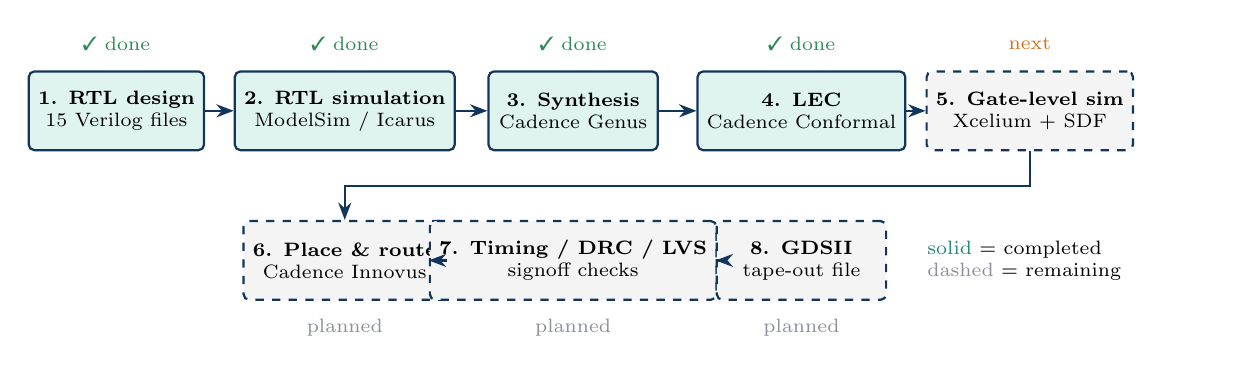
\begin{tikzpicture}[x=1cm,y=1cm]
    \tikzset{st/.style={minimum width=2.15cm,minimum height=1.0cm,rounded corners=2pt,thick,align=center,font=\scriptsize,draw=navy}}
    \node[st,fill=softteal] (a) at (0,0) {\textbf{1. RTL design}\\15 Verilog files};
    \node[st,fill=softteal] (b) at (2.9,0) {\textbf{2. RTL simulation}\\ModelSim / Icarus};
    \node[st,fill=softteal] (c) at (5.8,0) {\textbf{3. Synthesis}\\Cadence Genus};
    \node[st,fill=softteal] (d) at (8.7,0) {\textbf{4. LEC}\\Cadence Conformal};
    \node[st,fill=softgrey,dashed] (e) at (11.6,0) {\textbf{5. Gate-level sim}\\Xcelium + SDF};
    \node[st,fill=softgrey,dashed] (f) at (2.9,-1.9) {\textbf{6. Place \& route}\\Cadence Innovus};
    \node[st,fill=softgrey,dashed] (g) at (5.8,-1.9) {\textbf{7. Timing / DRC / LVS}\\signoff checks};
    \node[st,fill=softgrey,dashed] (h) at (8.7,-1.9) {\textbf{8. GDSII}\\tape-out file};
    \draw[arr] (a)--(b); \draw[arr] (b)--(c); \draw[arr] (c)--(d); \draw[arr] (d)--(e);
    \draw[arr] (e.south) |- ([yshift=0.0cm]f.north |- 0,-0.95) -- (f.north);
    \draw[arr] (f)--(g); \draw[arr] (g)--(h);
    \node[font=\scriptsize,good] at (0,0.85) {\ok\ done}; \node[font=\scriptsize,good] at (2.9,0.85) {\ok\ done};
    \node[font=\scriptsize,good] at (5.8,0.85) {\ok\ done}; \node[font=\scriptsize,good] at (8.7,0.85) {\ok\ done};
    \node[font=\scriptsize,orange] at (11.6,0.85) {next};
    \node[font=\scriptsize,midgrey] at (2.9,-2.75) {planned}; \node[font=\scriptsize,midgrey] at (5.8,-2.75) {planned}; \node[font=\scriptsize,midgrey] at (8.7,-2.75) {planned};
    \node[font=\scriptsize,align=left,text width=3.4cm] at (12.0,-1.9) {\textcolor{teal}{solid} = completed\\\textcolor{midgrey}{dashed} = remaining};
  \end{tikzpicture}
\end{frame}

% =============================================================================
\begin{frame}{Implementation details: tools, platforms and status}
  \footnotesize
  \renewcommand{\arraystretch}{1.18}
  \begin{tabularx}{\textwidth}{@{}p{3.1cm}p{4.7cm}Xp{1.6cm}@{}}
    \toprule
    \textbf{Stage} & \textbf{Tool / platform} & \textbf{Details} & \textbf{Status}\\
    \midrule
    Training & Python, PyTorch, scikit-learn & 64--16--10 MLP, UCI digits & \ok\ done\\
    Quantization \& compile & Python (NumPy), ONNX & INT8 weights, \py{prog.hex} (9,677 steps) & \ok\ done\\
    RTL design & Verilog-2001, 15 files & Parameterised $4{\times}4$ array, register bus + AXI4-Lite & \ok\ done\\
    Functional simulation & ModelSim (Windows), Icarus, Verilator & 0 mismatches, 0 timeouts & \ok\ done\\
    Driver & C (\py{driver/}) & Same register stream as the Python compiler & \ok\ done\\
    Synthesis & Cadence Genus 21.14, typical library, 10 ns clock & 75,624 cells, timing met & \ok\ done\\
    Equivalence check & Cadence Conformal LEC & RTL vs.\ netlist & \ok\ done\\
    Gate-level simulation & Cadence Xcelium & Netlist + cell models (+ SDF) & \todo\ next\\
    Place \& route, signoff & Cadence Innovus & Clock tree, routing, STA, DRC/LVS & \pend\ planned\\
    GDSII & Innovus / streamout & Final layout file & \pend\ planned\\
    \bottomrule
  \end{tabularx}
\end{frame}

% =============================================================================
\begin{frame}{Results (1): functional simulation}
  \begin{columns}[T]
    \begin{column}{0.5\textwidth}
      \shotbox{2.5cm}{ModelSim console: \texttt{*** PLAYER PASSED ***}\\(\texttt{9677 ops, 1313 reads, 0 mismatches, 0 timeouts})}{sim_console.png}
    \end{column}
    \begin{column}{0.5\textwidth}
      \shotbox{2.5cm}{ModelSim waveform: \texttt{clk}, \texttt{reg\_wr\_en}, \texttt{irq},\\controller state (LDW $\to$ COMP $\to$ DRAIN)}{sim_waveform.png}
    \end{column}
  \end{columns}
  \vspace{6pt}
  \begin{columns}[T]
    \begin{column}{0.5\textwidth}
      \shotbox{1.9cm}{Single-PE testbench: \texttt{tb\_pe PASSED} (15 checks)}{sim_pe.png}
    \end{column}
    \begin{column}{0.5\textwidth}
      \footnotesize\textbf{What the output means}
      \begin{itemize}\setlength{\itemsep}{1pt}
        \item \texttt{9677 ops}: steps replayed from \py{prog.hex}.
        \item \texttt{0 mismatches}: every checked read equals the Python reference.
        \item \texttt{0 timeouts}: the chip always finished.
        \item \texttt{PASSED} = hardware is bit-exact with the model.
      \end{itemize}
    \end{column}
  \end{columns}
\end{frame}

% =============================================================================
\begin{frame}{Results (2): accuracy and verification}
  \begin{columns}[T]
    \begin{column}{0.44\textwidth}
      \small\textbf{Accuracy on 360 unseen test images}\\[3pt]
      \renewcommand{\arraystretch}{1.25}
      \begin{tabular}{@{}lr@{}}
        \toprule
        \textbf{Model} & \textbf{Accuracy}\\
        \midrule
        Float (PyTorch) & 96.94\%\\
        INT8, Python golden & 96.94\%\\
        INT8, \textbf{on the RTL} & \textbf{96.94\%}\\
        \bottomrule
      \end{tabular}

      \vspace{8pt}
      
\begin{tikzpicture}
        \draw[navy!30] (0,0) rectangle (5.4,0.6);
        \fill[teal] (0,0) rectangle (5.4*0.9694,0.6);
        \node[white,font=\small\bfseries] at (2.6,0.3) {349 of 360 correct};
      \end{tikzpicture}

      \footnotesize Shrinking to INT8 and running on hardware cost \textbf{no accuracy}.
    \end{column}
    \begin{column}{0.54\textwidth}
      \small\textbf{Verification summary}\\[3pt]
      \footnotesize
      \renewcommand{\arraystretch}{1.25}
      \begin{tabularx}{\textwidth}{@{}Xl@{}}
        \toprule
        \textbf{Test} & \textbf{Result}\\
        \midrule
        Digit network, 45 batches (1,088 checked reads) & 0 mismatches\\
        Single PE testbench (15 checks) & PASS\\
        240 random networks, 7 configurations & ALL PASSED\\
        116 illegal-command tests & ALL PASSED\\
        AXI4-Lite bridge with random stalls & PASS\\
        C driver = Python register stream & PASS\\
        19 injected design faults (mutation test) & all caught\\
        \bottomrule
      \end{tabularx}
    \end{column}
  \end{columns}
\end{frame}

% =============================================================================
\begin{frame}{Results (3a): synthesis schematics (Cadence Genus)}
  \begin{columns}[T]
    \begin{column}{0.49\textwidth}
      \centering\shot{0.86\linewidth}{synthesis_pic1.png}\\[2pt]
      \footnotesize\textbf{Top level:} reset synchronizer, \texttt{dnn\_accel\_core}, \texttt{dnn\_reg\_if} and an OR gate that forms \texttt{irq}.
    \end{column}
    \begin{column}{0.49\textwidth}
      \centering\shot{0.86\linewidth}{synthesis_pic2.png}\\[2pt]
      \footnotesize\textbf{Reset synchronizer:} two flip-flops (reset asserts immediately, releases in step with the clock).
    \end{column}
  \end{columns}
  \vspace{4pt}
  \begin{block}{What to notice}
    \footnotesize\begin{itemize}\setlength{\itemsep}{1pt}
      \item The netlist has the same three blocks as the RTL hierarchy: reset sync, core, register interface.
      \item The register interface and the core talk through the wires between the two big boxes; the OR gate merges done and error into \texttt{irq}.
    \end{itemize}
  \end{block}
\end{frame}

\begin{frame}{Results (3b): synthesized blocks (Cadence Genus)}
  \begin{columns}[T]
    \begin{column}{0.49\textwidth}
      \centering\shot{0.86\linewidth}{synthesis_pic3.png}\\[2pt]
      \footnotesize\textbf{\texttt{u\_core} after mapping:} about 74,000 standard cells (flattened); contains the array, memories, controller and PPU.
    \end{column}
    \begin{column}{0.49\textwidth}
      \centering\shot{0.86\linewidth}{synthesis_pic4.png}\\[2pt]
      \footnotesize\textbf{\texttt{u\_if}:} the register interface (address decode, descriptor and status registers).
    \end{column}
  \end{columns}
  \vspace{4pt}
  \begin{block}{What to notice}
    \footnotesize\begin{itemize}\setlength{\itemsep}{1pt}
      \item \texttt{u\_core} is flattened: array, memories, controller and PPU are mapped to about 74,000 gates and flip-flops.
      \item \texttt{u\_if} is small (about 1,200 cells): address decoding plus the descriptor and status registers.
    \end{itemize}
  \end{block}
\end{frame}

% =============================================================================
\begin{frame}{Results (4): synthesis reports --- timing and power}
  \begin{columns}[T]
    \begin{column}{0.5\textwidth}
      \begin{block}{Timing (clock 10 ns = 100 MHz)}
        \footnotesize
        \renewcommand{\arraystretch}{1.15}
        \begin{tabular}{@{}lr@{}}
          \toprule
          Setup slack & \textbf{+1,144 ps (MET)}\\
          Data path delay & 8,662 ps\\
          Setup time / uncertainty & 94 ps / 100 ps\\
          Estimated max.\ clock & $\approx$ 113 MHz\\
          \bottomrule
        \end{tabular}\\[3pt]
        \scriptsize Critical path: control register $\to$ PPU rounding adder $\to$ shift $\to$ clamp $\to$ output register.
        Conditions: typical, wireload \emph{enclosed}, ideal clock.
      \end{block}
    \end{column}
    \begin{column}{0.48\textwidth}
      \begin{block}{Power (no switching-activity file)}
        \footnotesize
        \renewcommand{\arraystretch}{1.15}
        \begin{tabular}{@{}lrr@{}}
          \toprule
          \textbf{Component} & \textbf{mW} & \textbf{Share}\\
          \midrule
          Leakage & 5.43 & 7.95\%\\
          Internal & 60.48 & 88.53\%\\
          Switching & 2.40 & 3.52\%\\
          \midrule
          \textbf{Total} & \textbf{68.3} & 100\%\\
          \bottomrule
        \end{tabular}\\[3pt]
        \scriptsize Registers 91.3\%, logic 8.7\%. Clock-tree power not included (ideal clock).
      \end{block}
    \end{column}
  \end{columns}
  \vspace{2pt}
  \scriptsize\emph{Pre-layout estimates: wires, clock tree and real switching activity will change the numbers after place and route.}
\end{frame}

% =============================================================================
\begin{frame}{Results (5): synthesis report --- area}
  \begin{columns}[T]
    \begin{column}{0.5\textwidth}
      \footnotesize
      \renewcommand{\arraystretch}{1.12}
      \begin{tabular}{@{}lrrr@{}}
        \toprule
        \textbf{Block} & \textbf{Cells} & \textbf{Area} & \textbf{\%}\\
        \midrule
        \textbf{dnn\_accel\_top} & 75,624 & 953,673 & 100\\
        \quad Weight + act.\ SRAM + ctrl$^{*}$ & -- & 663,085 & 69.5\\
        \quad Accumulator SRAM & 5,951 & 114,452 & 12.0\\
        \quad Bias SRAM & 3,101 & 58,425 & 6.1\\
        \quad PPU & 6,560 & 55,825 & 5.9\\
        \quad Systolic core (array+skew) & 4,778 & 38,804 & 4.1\\
        \quad Register interface & 1,209 & 10,466 & 1.1\\
        \quad LRB & 616 & 8,048 & 0.8\\
        \quad Perf counters & 689 & 4,522 & 0.5\\
        \quad Reset sync & 2 & 41 & $\approx$0\\
        \bottomrule
      \end{tabular}\\[2pt]
      \tiny $^{*}$ flattened into \texttt{u\_core}; obtained as u\_core minus the listed sub-blocks. Area in library units.
    \end{column}
    \begin{column}{0.48\textwidth}
      \centering
      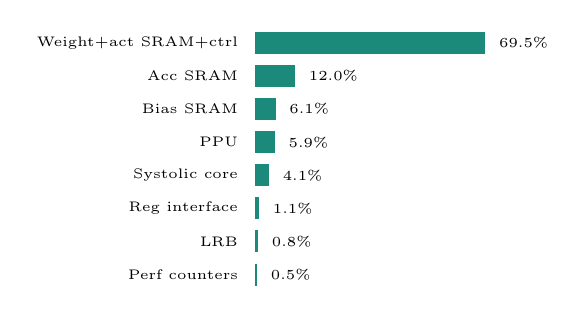
\begin{tikzpicture}[x=1cm,y=1cm]
        \def\bars{{69.5,12.0,6.1,5.9,4.1,1.1,0.8,0.5}}
        \foreach \v/\n [count=\i from 0] in {69.5/Weight+act SRAM+ctrl,12.0/Acc SRAM,6.1/Bias SRAM,5.9/PPU,4.1/Systolic core,1.1/Reg interface,0.8/LRB,0.5/Perf counters}{
          \node[anchor=east,font=\tiny] at (1.55,-\i*0.42) {\n};
          \fill[teal] (1.65,-\i*0.42-0.14) rectangle ++(\v*0.042,0.28);
          \node[anchor=west,font=\tiny] at (1.7+\v*0.042,-\i*0.42) {\v\%};
        }
      \end{tikzpicture}

      \footnotesize\textbf{Why so large?} The SRAMs are currently built from flip-flops, since no memory macros were used. Real SRAM macros from the foundry would shrink this a lot.
      Total flip-flops: $\approx$ 33,657.
    \end{column}
  \end{columns}
\end{frame}

% =============================================================================
\begin{frame}{Results (6a): logic equivalence check (Cadence Conformal)}
  \begin{columns}[T]
    \begin{column}{0.49\textwidth}
      \centering\shot{0.86\linewidth}{lec_main.png}\\[2pt]
      \footnotesize\textbf{Golden} (RTL) vs.\ \textbf{Revised} (Genus netlist): same hierarchy; the log ends with ``Compare done''.
    \end{column}
    \begin{column}{0.49\textwidth}
      \centering\shot{0.86\linewidth}{lec_mapping.png}\\[2pt]
      \footnotesize\textbf{Mapping manager:} no unmapped points; the compared points (e.g.\ \texttt{reg\_rdata[\ldots]}) are marked equivalent.
    \end{column}
  \end{columns}
  \vspace{4pt}
  \begin{block}{How to read it}
    \footnotesize\begin{itemize}\setlength{\itemsep}{1pt}
      \item \textbf{Golden} = our RTL; \textbf{Revised} = the gate netlist written by Genus. The tool maps every input, output and flip-flop of one to the other.
      \item \textbf{Mapped points:} inputs such as \texttt{clk}, \texttt{reg\_addr}; \textbf{compared points:} outputs and registers whose logic is proven equal.
    \end{itemize}
  \end{block}
\end{frame}

\begin{frame}{Results (6b): equivalence check --- schematics and meaning}
  \begin{columns}[T]
    \begin{column}{0.55\textwidth}
      \centering\shot{\linewidth}{lec_schematics.png}\\[2pt]
      \footnotesize Simplified schematics of the golden (left) and revised (right) designs.
    \end{column}
    \begin{column}{0.43\textwidth}
      \begin{block}{What LEC proves}
        \footnotesize The synthesized gate netlist is \textbf{logically identical} to the RTL for \emph{every possible input}
        --- a mathematical proof, not a test. So synthesis did not change what the design does.
        %%% EDIT %%% add the final summary line from Conformal here (number of equivalent points, 0 non-equivalent)
      \end{block}
    \end{column}
  \end{columns}
\end{frame}

% =============================================================================
\begin{frame}{Tabulation: key numbers at a glance}
  \footnotesize
  \renewcommand{\arraystretch}{1.15}
  \begin{columns}[T]
    \begin{column}{0.49\textwidth}
      \begin{tabular}{@{}lr@{}}
        \toprule
        \textbf{Design / performance} & \textbf{Value}\\
        \midrule
        Array / precision & 4$\times$4, INT8\\
        Network & 64 $\to$ 16 $\to$ 10\\
        Weights + biases & 1,184 + 26\\
        Cycles per batch of 8 & 1,771\\
        Throughput @ 100 MHz & $\approx$ 452,000 images/s\\
        Compute rate & $\approx$ 1.07 GOPS\\
        Peak MACs / clock & 16\\
        Array utilisation & 33.4\%\\
        \bottomrule
      \end{tabular}
    \end{column}
    \begin{column}{0.49\textwidth}
      \begin{tabular}{@{}lr@{}}
        \toprule
        \textbf{Implementation} & \textbf{Value}\\
        \midrule
        Verilog files / pins & 15 / 85\\
        Std cells (synthesis) & 75,624\\
        Area (library units) & 953,673\\
        Setup slack @ 10 ns & +1,144 ps\\
        Power (estimate) & 68.3 mW\\
        Efficiency (estimate) & $\approx$ 15.7 GOPS/W\\
        Accuracy on RTL & 96.94\%\\
        \bottomrule
      \end{tabular}
    \end{column}
  \end{columns}
  \vspace{6pt}

  \begin{block}{Effect of the local reuse buffer (per batch of 8)}
    \footnotesize
    \begin{tabularx}{\textwidth}{@{}Xrr@{}}
      \toprule
      & \textbf{Without LRB} & \textbf{With LRB}\\
      \midrule
      Activation SRAM reads & 608 words & \textbf{160 words} (3.8$\times$ fewer)\\
      Activation fetches served by LRB & 0\% & 73.7\%\\
      \bottomrule
    \end{tabularx}
  \end{block}
  \tiny GOPS = 2 operations per MAC $\times$ 1,184 MACs $\times$ images/s; efficiency = GOPS / power (pre-layout power, no activity file).
\end{frame}

% =============================================================================
\begin{frame}{Observations and honest limitations}
  \begin{columns}[T]
    \begin{column}{0.49\textwidth}
      \begin{block}{What went well}
        \footnotesize
        \begin{itemize}\setlength{\itemsep}{2pt}
          \item Hardware is bit-exact with the Python model; no accuracy lost to INT8.
          \item Timing is met with margin (+1.14 ns at 100 MHz).
          \item LEC confirms synthesis preserved the logic.
          \item LRB cuts activation reads by 3.8$\times$.
        \end{itemize}
      \end{block}
    \end{column}
    \begin{column}{0.49\textwidth}
      \begin{block}{What we will improve}
        \footnotesize
        \begin{itemize}\setlength{\itemsep}{2pt}
          \item \textbf{Area:} memories are flip-flops $\Rightarrow$ move to SRAM macros.
          \item \textbf{Timing:} critical path is the PPU rounding adder $\Rightarrow$ pipeline / faster adder.
          \item \textbf{Utilisation:} array is busy 33\% of the time $\Rightarrow$ overlap load and compute.
          \item \textbf{Power:} re-estimate after clock tree and with real activity.
          \item \textbf{Testability:} scan-chain (DFT) insertion is future work.
        \end{itemize}
      \end{block}
    \end{column}
  \end{columns}
\end{frame}

% =============================================================================
\begin{frame}{Demonstration of working modules}
  \begin{columns}[T]
    \begin{column}{0.5\textwidth}
      \shotbox{3.0cm}{Demo video / screen recording:\\running \texttt{run\_modelsim.bat} $\to$ \texttt{PASSED}\\\scriptsize(add a link or QR code here)}{demo_video_link}
    \end{column}
    \begin{column}{0.5\textwidth}
      \footnotesize\textbf{Suggested live demo (3 steps)}
      \begin{enumerate}\setlength{\itemsep}{2pt}
        \item \py{show_digits.py}: show the test pictures.
        \item Run the simulation (\py{run_modelsim.bat}): see \texttt{PLAYER PASSED}.
        \item \py{compare_one.py 17}: chip scores and Python scores side by side --- identical; biggest score = predicted digit.
      \end{enumerate}
    \end{column}
  \end{columns}
\end{frame}

% =============================================================================
\begin{frame}{Research objective -- SDG alignment}
  \footnotesize
  \renewcommand{\arraystretch}{1.25}
  \begin{tabularx}{\textwidth}{@{}p{3.6cm}p{4.9cm}X@{}}
    \toprule
    \textbf{UN Sustainable Development Goal} & \textbf{Target} & \textbf{Link to this project}\\
    \midrule
    \textbf{SDG 9} \,Industry, Innovation \& Infrastructure &
      9.5 Enhance scientific research and upgrade technological capabilities &
      Indigenous, fully documented AI-accelerator ASIC design flow; builds chip-design capability.\\
    \textbf{SDG 7} \,Affordable \& Clean Energy &
      7.3 Double the global rate of improvement in energy efficiency &
      Dedicated INT8 hardware with data reuse uses far less energy per inference than a general processor.\\
    \bottomrule
  \end{tabularx}
  \vspace{4pt}

  \scriptsize\emph{Please confirm the exact SDGs/targets your department expects before the review.}
\end{frame}

% =============================================================================
\begin{frame}{Timeline plan: remaining milestones}
  \centering
  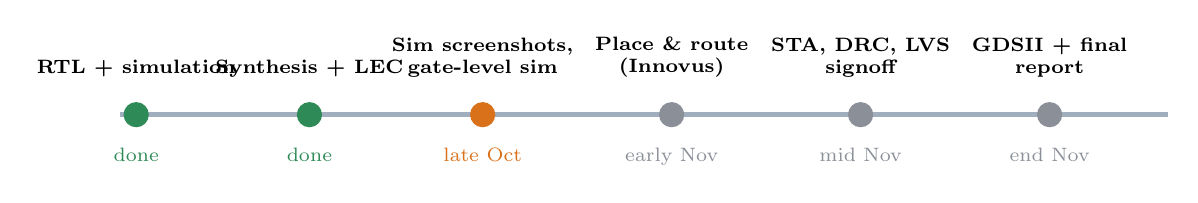
\begin{tikzpicture}[x=1cm,y=1cm]
    \draw[ultra thick,navy!40] (0,0) -- (13.3,0);
    \foreach \x/\t/\d/\c in {0.2/{RTL + simulation}/{done}/good, 2.4/{Synthesis + LEC}/{done}/good, 4.6/{Sim screenshots,\\gate-level sim}/{late Oct}/orange, 7.0/{Place \& route\\(Innovus)}/{early Nov}/midgrey, 9.4/{STA, DRC, LVS\\signoff}/{mid Nov}/midgrey, 11.8/{GDSII + final\\report}/{end Nov}/midgrey}{
      \fill[\c] (\x,0) circle (0.16);
      \node[font=\scriptsize\bfseries,align=center,anchor=south] at (\x,0.35) {\t};
      \node[font=\scriptsize,anchor=north,\c] at (\x,-0.3) {\d};
    }
  \end{tikzpicture}

  \vspace{6pt}
  \footnotesize
  \renewcommand{\arraystretch}{1.15}
  \begin{tabularx}{\textwidth}{@{}p{3.3cm}Xp{2.4cm}@{}}
    \toprule
    \textbf{Milestone} & \textbf{Deliverable} & \textbf{Target}\\
    \midrule
    Gate-level simulation & Netlist passes \py{tb_dnn_player} (0 mismatches) & late Oct\\
    Netlist improvements & Memory macros, PPU timing fix (optional) & early Nov\\
    Place \& route & Clock tree, routing, post-layout timing/power & early Nov\\
    Signoff & Timing, DRC, LVS clean & mid Nov\\
    Final deliverables & GDSII, project report, presentation & end Nov\\
    \bottomrule
  \end{tabularx}
  \vspace{3pt}\tiny\emph{Dates are proposed; adjust to the department's schedule.}
\end{frame}

% =============================================================================
\begin{frame}{Conclusion}
  \begin{columns}[T]
    \begin{column}{0.55\textwidth}
      \begin{block}{Summary}
        \small
        \begin{itemize}\setlength{\itemsep}{3pt}
          \item A compact, programmable INT8 systolic-array DNN accelerator is designed in 15 Verilog files.
          \item It runs a digit-recognition network at \textbf{96.94\%} accuracy, bit-exact with the Python reference.
          \item Synthesis: 75,624 cells, \textbf{timing met} at 100 MHz, $\approx$ 68 mW (pre-layout).
          \item \textbf{LEC} confirms the netlist matches the RTL.
        \end{itemize}
      \end{block}
    \end{column}
    \begin{column}{0.42\textwidth}
      \begin{block}{Next}
        \small
        \begin{itemize}\setlength{\itemsep}{3pt}
          \item Gate-level simulation
          \item Place \& route with Innovus
          \item Signoff checks and GDSII
          \item Optional: SRAM macros, DFT, PPU timing
        \end{itemize}
      \end{block}
    \end{column}
  \end{columns}
\end{frame}

% =============================================================================
\begin{frame}{References}
  \footnotesize
  \begin{enumerate}\setlength{\itemsep}{3pt}
    \item H.\,T.\ Kung, ``Why systolic architectures?'', \emph{IEEE Computer}, vol.\ 15, no.\ 1, 1982.
    \item N.\ P.\ Jouppi et al., ``In-datacenter performance analysis of a Tensor Processing Unit'', \emph{ISCA}, 2017.
    \item Y.-H.\ Chen, T.\ Krishna, J.\ Emer, V.\ Sze, ``Eyeriss: An energy-efficient reconfigurable accelerator for deep convolutional neural networks'', \emph{IEEE JSSC}, 2017.
    \item V.\ Sze, Y.-H.\ Chen, T.-J.\ Yang, J.\ Emer, ``Efficient processing of deep neural networks: A tutorial and survey'', \emph{Proc.\ IEEE}, 2017.
    \item B.\ Jacob et al., ``Quantization and training of neural networks for efficient integer-arithmetic-only inference'', \emph{CVPR}, 2018.
    \item H.\ Genc et al., ``Gemmini: Enabling systematic deep-learning architecture evaluation via full-stack integration'', \emph{DAC}, 2021.
    \item E.\ Alpaydin, C.\ Kaynak, ``Optical Recognition of Handwritten Digits'', UCI Machine Learning Repository, 1998. DOI 10.24432/C50P49.
    \item Cadence Genus, Conformal LEC, Innovus and Xcelium user documentation.
  \end{enumerate}
\end{frame}

% =============================================================================
\begin{frame}[plain]
  \begin{tikzpicture}[remember picture,overlay]
    \fill[navy] (current page.south west) rectangle (current page.north east);
    \node[text=white,font=\bfseries\Huge] at (current page.center) {Thank you};
    \node[text=white!80!navy,font=\Large] at ([yshift=-1.2cm]current page.center) {Questions?};
  \end{tikzpicture}
\end{frame}

\end{document}
